\section{Wprowadzenie Teoretyczne}

\subsection{Sieci bezprzewodowe krotkiego zasiegu}

\par
\tab Bezprzewodowe sieci krótkiego zasięgu są dzielone na dwie grupy WLANs (Wireless local area networks) i WPANs(Wireless personal area networks). Jak sama nazwa wskazuje sieci WLAN są bezprzewodowym zamiennikiem lub rozszeżeniem dla sieci przewodowych typu LAN (Local area network) dzięki czemu urządzenia wchodzące w skład sieci WLAN mogą być łatwo zintegrowane z przedowodymi sieciami LAN.
\\
\par
Sieci WPAN natomiast powstały w zupełnie innym zamyśle i od swoich początków były tworzone jako oddzielne-niezależne służące energo-oszczędnej komunikacji bezprzewodowej na obszarze tzw. POS (Personal operating space) który to jest niezależny od żadnej innej infrastruktury.
\\
\par
Zgrubny podział sieci krótkiego zasięgu przedstawia poniższy schemat:\\
\\
\centerline{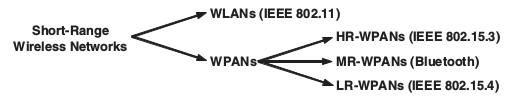
\includegraphics[scale=0.5]{./img/img_0__2_1}}
\\
\par 
Sieci typu WPAN możemy podzielić na 3 grupy: \\
\tab Sieci HR (high-rate) o wysokiej przepustowości danych, MR (medium-rate) sieci o umiarkowanej przepustowości oraz LR (low-rate) sieci o niskiej przepustowości. \\
\tab Przykładem sieci o wysokiej przepustowości może być siec służąca do streamingu w czasie rzeczywistym z kamery do HD-TV (jest to typowe zastosowanie standardu HR-WPAN IEEE 802.15.3), taki transfer sięga do prawie 60Mbs. Typowym reprezentantem sieci MR są rozwiązania oparte o Bluetooth z transferem sięgającym do 3Mbps który może służyć np. do wysokiej jakości transmisji głosowej. W skład ostatniej grupy LR wchodzi protokół ZigBee z maxymalną prędkością transferu sięgającą 250Kbps. \\


\clearpage
